\documentclass{llncs}
\usepackage{makeidx}  % allows for indexgeneration
\usepackage[pdftex]{graphicx} % PNGs
\usepackage{amsmath, amssymb} % algebra
\usepackage[utf8x]{inputenc}
\usepackage[T1]{fontenc} 
\usepackage[procnames]{listings} % for sourcecode
\usepackage{graphviz} % graphs
\usepackage{array,multirow} % tables
\usepackage{afterpage} % figures
\usepackage{float} % figures

\lstset{%
	basicstyle=\small\ttfamily,
	sensitive=true,
	keywordsprefix=P,
	keywords={END,W,W1},
	keywordstyle=\bfseries,
	identifierstyle=\ttfamily,
	procnamestyle=\bfseries,
	procnamekeys={P},
	numbers=left,
	literate={<}{$<$}1 {>}{$>$}1 {=}{$=$}1 {<=}{$\leq$}1 {>=}{$\geq$}1 {=>}{{$\Rightarrow$}}1 {->}{{$\rightarrow$}}1,
	frame=lines,
	numbers=left,
	numberstyle=\rmfamily\tiny,
	numbersep=3pt,
	breaklines=true,
	breakatwhitespace=true
}

\restylefloat{figure}
\begin{document}
\pagestyle{headings}  % switches on printing of running heads
\mainmatter % start of the contributions
\title{The Plankalkül}
\subtitle{An Early High-Level Programming Language}
\titlerunning{The Plankalkül}  % abbreviated title (for running head)
\author{Tim Felgentreff}
\date{\today}
\authorrunning{Tim Felgentreff}   % abbreviated author list (for running head)
\tocauthor{Tim Felgentreff (Hasso-Plattner-Institute)}
\institute{History of Programming Languages, Software Architecture Group, Hasso-Plattner-Institut, Universität Potsdam, D-14482 Potsdam, Germany,\\
\email{tim.felgentreff@student.hpi.uni-potsdam.de}}

\maketitle
\begin{abstract}
   Lectures on the history of computing have for a long time 
   ignored any development on the matter before the end of World War II. 
   This for a long time supported the view that the roots of 
   computing and programming languages lie with large corporations 
   like IBM and the Universities.
   Although today
   the German engineer Konrad Zuse is widely recognised
   as the first inventor of general purpose computing machines, 
   and his automatons are widely explored, another invention of 
   his, the very first concept of a 
   high-level programming language, has remained largely unheard of.
   This paper explores Zuse's language, ``Der Plankalkül'', 
   and describes some its background and concepts, as well as its 
   meaning for the history of programming languages.
\end{abstract}
 \section{Introduction}
   Most people working with computers on a professional level have
   at some time heard of Konrad Zuse and his Z3, the first fully 
   automatic programmable computer. This computer, built in the 
   house of his parents, from old phone relays, by a man who has had no 
   previous contact with other scientists working on automatic computation, 
   has been so thoroughly reviewed and been written about, that it 
   stands synonym for Konrad Zuse's life work.

   However, parallel to his efforts on building the Z1 through Z3, Zuse
   also worked on his programming language, which he called ``Plan Calculus''
   to show its sources in the ``logical calculus''. The first notes about
   this language appeared in his notebooks in May, 1939~\cite{rojas2002konrad}. The \emph{Genesis}
   of the Plankalkül lies in the years 1942 to 45.

   In this paper we will elaborate on the historical background in which 
   Zuse conducted his work, as well as explore earlier and parallel attempts 
   at similar work. After exploring Zuse's incentive for creating a programming 
   language, we will present his Plan Calculus in more detail, giving an overview 
   of its syntax and data-structures as well as its higher-level constructs and compare 
   those to modern programming languages. Finally, we consider the impact Zuse
   had with his language on the popular programming languages which came after.
 \section{History}
   Work on mechanical calculation goes back to the invention of the Abacus, but one 
   of the first notable ``computing'' machines was Charles Babbage's \emph{Analytical Engine},
   which he first described in 1837. It was for this theoretical machine (which was not built until the 
   late 1960s), that Ada Lovelace later wrote an instruction set for calculating the Bernoulli numbers\cite{hyman1985Charles}.
   These instructions, written in an assembly-like language, are today considered the very first computer program.

   Due to lack of interest and money, the \emph{Engine} was never built and the next 
   time somebody should concern himself with computation in such depth was 
   one hundred years later. During the 1930s, one Alan Turing started his work on computable numbers\cite{turing1936computable}
   and Konrad Zuse began working on his Z1.
 \subsection{Zuse and Computing}
   Konrad Zuse was a civil engineer in the Germany of the 1920s. He became annoyed by
   the repetitive nature of the computations he had to perform at his workplace and began to 
   to consider building machines to perform such dull computations.
   Due to his engineering background he had never come in contact with previous 
   ideas of the kind and the political developments at the time kept him 
   from exploring parallel developments in the United States at the time. He did not learn
   about Babbage's work until after his machines were built and he had patents on them\cite{epegmagHorstzuse}.

   To work on his first machine, the V1 (later renamed to Z1, not to be 
   confused with the V-line of German rockets), Zuse borrowed money
   from friends and relatives. He built the Z1 at his parents home, cutting the 
   pieces he needed with a jigsaw. We know today that his design would have worked,
   but the rough nature of the parts the computer was built of made it extremely unreliable,
   and so Zuse notes in May, 1939: ``Rechenwerk fertig, aber funktioniert schlecht''\cite{rojas2002plankalkuel}.
 \subsection{The Z1 to Z4}
   Working almost completely on his own, Zuse designed and built machines 
   which had many characteristics of todays computers. All his machines
   had binary floating-point arithmetics, separate \emph{Arithmetic logic units} (ALU), 
   a central processor and general purpose memory banks.
   Programs were written on punched tape and his Z1 and Z3 had 24bit word-sizes
   and arithmetic exception handling. A scheme if the Z1 can be seen in Fig.\ref{fig:z1}.
   
  \begin{figure}[t]
    \centering
    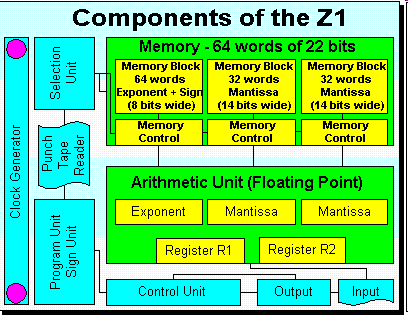
\includegraphics[width=0.5\linewidth]{img/z1.png}
    \caption{Top-down view of the Z1\cite{epegmagHorstzuse}}
    \label{fig:z1}
  \end{figure}

   Zuse basically created the von Neumann architecture (without saving the program to memory)
   before it was even formulated\cite{epegmagHorstzuse} 
   and invented a notation which he called ``combinatorics of conditionals'' which was
   identical to the propositional calculus, as Zuse himself realized later.
 \subsection{The Vision of a Chess Game}
   Zuse knew the potential of his machine. He told his co-workers and 
   friends, that one day, he would teach it to play a game of chess 
   against him. However, on trying to create an implementation, he realized 
   that ``even simple relations are very difficult to express''. In the course
   of the second World War, Konrad Zuse was able to avoid the army and 
   continue his work. 
   
   Zuse concerned himself with problems that engineers and scientists needed to 
   solve. He learned about the concepts of boolean algebra and found many 
   of his ideas reflected in it. He derived, that any problem was expressible
   using only the basic operations NOT, AND and OR. He developed this epiphany 
   to conceptually create a \emph{logistic machine} (Fig. \ref{fig:logicmachine}), 
   as opposed to algebraic machines such as his Z1, Z2 and Z3\cite{epegmagHorstzuse}.
   
   Konrad Zuse knew
   that from simple building blocks, as were his logistic machines, 
   he could create hierarchical structures that would be able to solve any 
   computationally solvable problem. Interestingly, he already considered the chess game as
   benchmark for the capabilities of his machines\cite{rojas2002konrad}.
 \section{The Plankalkül}
   While initially only meant as a descriptive language, Zuse gradually 
   developed a possible implementation as a programming language, especially 
   after he was no longer able to work on his machines through the events of the war\cite{giloi2002konrad}.
   In this process he added explicit constructs to the implicit notation and developed ideas 
   on how to map those formulas onto computers\cite{rojas2002konrad}.
 \subsection{Motivation}
  \begin{figure}[bt]
    \centering
    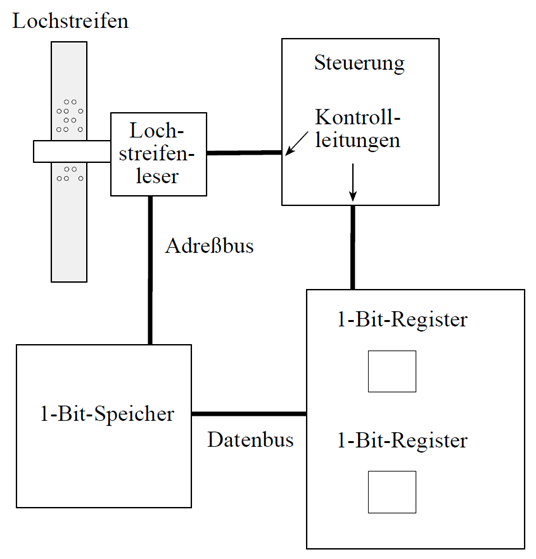
\includegraphics[width=0.4\linewidth]{img/logicmachine.png}
    \caption{A scheme of Zuse's \emph{logic machine}\cite{rojas2002plankalkuel}}
    \label{fig:logicmachine}
  \end{figure}

   Zuse had realized early on, through his study of propositional logic, that any 
   logical statement could be mapped onto his logistic machine. His Plan Calculus
   allows high level programming even for simple hardware and worked to the mind 
   of the programmer with variables, conditions and re-usable subcomponents\cite{giloi2002konrad}.
 \subsection{Basic Concepts}
   In the following we would like to present some of 
   the concepts which can be found in the Plankalkül 
   and provide reasons for them, were they seem far-fetched 
   or surprising.
   
   When considering Konrad Zuse's language, we have to keep 
   in mind his hardware development background. While Zuse strived 
   to create a universial language that made it easy to write 
   programs for his computers, he eventually meant for them to
   be converted into basic statements to run on hierarchies of 
   his logistic machines. Even as such, the Plan Calculus is in some aspects more
   expressive than early languages like ALGOL or FORTRAN and had more 
   concepts alike with the mathematical language APL\cite{giloi2002konrad}
   
   From the start, Zuse realized that all computation can be expressed 
   in the form $F(x) \Rightarrow R$. He considered computing in a very 
   general sense, writing in his notes: ``Rechnen heißt: Aus
   gegebenen Angaben nach einer Vorschrift neue Angaben bilden''\cite{bauer1972plankalkuel}

   Additionally, Zuse decided to use the binary 
   true/false logic as most basic type. While many modern languages still 
   do not have a bit type (e.g. C, C++), use of the binary system as such 
   for algebra was not even widely explored at the time. As late as 1938 Bell Labs created a 
   research program for the matter, something Zuse did not know of. The first 
   language after the Plankalkül to implement a binary data type for use in 
   boolean logic was ALGOL 60.
   
   Those basic ideas, while noteworthy, do not make the language any more
   high-level than the weaving descriptions of one Ada Lovelace. 
   Zuse intended his language to have a much stronger expressibility. 
   Especially in hindsight it is remarkable 
   to what extend Zuse already considered standard features of modern 
   programming languages for his Plan Calculus.
   
   \begin{description}
     \item[GOTO] Der Plankalkül does not have 
       a GOTO statement. While this may be due to some excellent
       foresight of Zuse's, the GOTO statement would also be
       difficult to implement with punched tape.
     \item[Call by Value] Call by Value is parameter passing mode 
       where the parameter is essentially copied to the function because
       writing to the input variables is denied. This is very natural 
       and eases debugging as side effects happen before calls.
     \item[No Recursion] 
       The ideas of Zuse's hierarchically structured machines would not 
       allow implementation of such behavior in hardware without resorting 
       to some kind of hardware stack.
     \item[Loops] The Plan Calculus has a powerful loop statement, 
       which can be used either like a modern limited loop (for-to) 
       or a conditional loop (while). This made the language Turing
       complete even though Zuse neither knew the term nor the 
       concept at the time.
     \item[Branches] Conditional branching was already implemented 
       in the Z3 and the concept was included in his calculus, too.
     \item[Algebraic Notation] Konrad Zuse derived his program 
       notation from the propositional calculus which makes
       it more natural to read for the programmer than assembler like 
       language.
   \end{description}
   These concepts are reasons for considering Der Plankalkül a
   high-level programming language. They are explained in more detail 
   in the following sections.
 \subsection{Notation}
 \begin{figure}[tb]
   \begin{center}
     \begin{tabular}[bt]{c c c c c c c | c}
       V & + & V & $\Rightarrow$ & Z & {\LARGE\multirow{3}{*}{$\swarrow$}} & Z & ~\\
       0 &   & 1 &               & 1 &   & 0 & {\bf V}\\
       1 &   &   &               &   & &   & {\bf K}\\
       2.0 & & 2.0 &             & 2.0 & & 0 & {\bf S} \\
       \multicolumn{3}{c}{$\underbrace{\qquad\qquad}_{\text{Addition}}$}
       	& & \multicolumn{3}{c}{$\underbrace{\qquad\qquad\quad}_{\text{Dynamic select}}$} \\
	\multicolumn{7}{c}{$\underbrace{\qquad\qquad\qquad\qquad}_{\text{Assignment}}$} &
     \end{tabular}
   \end{center}
   \caption{The Tabular Notation of the Plan Calculus}
   \label{fig:notation}
 \end{figure}
   Certainly one of the most obvious deviations from almost all other programming 
   languages is the tabular notation Zuse chose to write his ``Program Plans'' in\ref{fig:notation}. 
   
   Almost all programming languages that came afterwards were designed with the input
   methods already thought out. Zuse approached his language without being preoccupied 
   with common input methods simply for the reason that there were none. So he chose 
   to represent programs in the Plan Calculus in statements consisting of four lines. 
   The main line includes the statement essentially in its mathematical form, 
   e.g. operations, conditions or variable assignments.
   The second line, which Zuse called the \emph{Variable Line}, is used to identify 
   the variable by a subindex. The S-line, called \emph{Structure Line}, denotes the 
   structure inside the variable which determines its \emph{type}. In the example above, the variables 
   $\binom{V}{0}$, $\binom{V}{1}$ and $\binom{Z}{1}$ are of type 2.0, and the variable $\binom{Z}{0}$
   has the simple type 0. In Zuse's examples the S-line is not always filled, especially when the 
   type of a variable is clear from the context, however, he notes that it simplifies understanding 
   of the formula\cite{bauer1972plankalkuel}.\\
   The K, or \emph{Component Line}, can be used to select only parts of a variables structure to operate 
   on.
 \subsection{Variables}
   Above we have seen the use of two types of variables, the Z and the V type. The Z variables are 
   used to hold the intermediate values of calculations, they could be written to and read from, while 
   V variables can only be read and were used as arguments passed to subroutines. There is a third kind, 
   the R variables, which can only be written to and are used to return data from a subroutine.

   This distinction between variable types is unusual in modern programming languages, but maps 
   very nicely onto the mechanical execution mechanisms Zuse worked with.
 \subsubsection{Types}
   \begin{figure}[tb]
     \begin{center}
       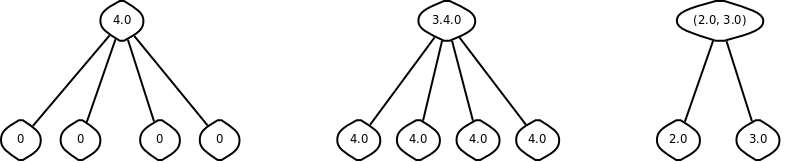
\includegraphics[width=\linewidth]{img/trees}
     \end{center}
     \caption{Variable Structure Trees}
     \label{fig:trees}
   \end{figure}
   Through the structure of his variables, Zuse, building on the simple data type Bit, was able
   to use data types like floating and fixed point, arrays and complex numbers\cite{epegmagHorstzuse}. 
   The dotted notation can be interpreted as a tree of memory cells (Fig. \ref{fig:trees}). 
   Types could be composed from arrays or tuples of other types. The only difference between the two 
   is that in arrays all leaves are of the same type whereas tuples can be composed of different 
   types. Figure \ref{fig:trees} shows two arrays of type 4.0 and 3.4.0 as well as a tuple type 
   composed of the two array types 2.0 and 3.0. Using the K line, the programmer is able to choose
   an arbitrary node in the tree to operate on, which comes close to the ideas of \emph{structs} in
   the C programming language or \emph{fields} within objects in object-oriented languages.
 \subsection{Higher-level constructs}
   Through his studies of engineering problems, Zuse identified many points of variation 
   which would be useful to solve a given problem. ``Der Plankalkül'' is a very dynamic 
   programming language. One interesting characteristic can already be seen in Fig. \ref{fig:notation}: 
   the variable Z0 determines the value in the K line for Z1, thus allowing dynamic choice of 
   different parts of the structure of Z1\cite{zuse1948allgemeinen}.
   \begin{figure}[h!]
     \begin{center}
       \begin{tabular}[bt]{c c c c c c c | c}
	 V & > & V & $\rightarrow$ & Z & $\Rightarrow$ & Z & ~\\
	 0 &   & 1 &               & 1 &               & 0 & {\bf V}\\
	 1 &   &   &               &   &               &   & {\bf K}\\
	 2.0 & & 2.0 &             & 0 &               & 0 & {\bf S}\\
       \end{tabular}
     \end{center}
     \caption{Conditional Execution}
     \label{fig:ifthen}
   \end{figure}
   The conditional execution depicted in Fig. \ref{fig:ifthen} assigns the value of Z1 to Z0 if
   the value in V0 is larger than V1. Note that there is no need for brackets 
   here, as Zuse uses the operator precedence of the predicate logic. Noteworthy 
   is the use of the implication arrow for conditional execution, which shows 
   the Plan Calculus' roots in the predicate calculus.
   \begin{equation*}
     \begin{matrix} 
       \text{W}~\\~\\~\\~\\~\\
     \end{matrix}
     \left[ \begin{matrix}
       \text{C1}\rightarrow\text{S1}\\
       \text{C2}\rightarrow\text{S2}\\
       \text{C3}\rightarrow\text{S3}\\
       \text{C4}\rightarrow\text{S4}\\
       \text{C5}\rightarrow\text{S5}
     \end{matrix} \right]
     \label{eq:while}
   \end{equation*}
   ``Der Plankalkül'' has loops, but no GOTO statement. A loop is started with a $W$ and followed
   by a $[block]$. This block includes conditional statements, and is repeated until all of the 
   statements are false, or a $FIN$ is called. The loop in Fig. \ref{eq:while} is executed as long 
   as at least one of the statements C1 to C5 evaluates to true. Blocks can be nested, then the $W$'s 
   have to be assigned indices as in:
   \begin{equation*}
     \begin{matrix}\text{W1}\\0\end{matrix}\left[ \dots 
     \begin{matrix}\text{W1}\\1\end{matrix} \left[ \dots 
     \begin{matrix}\text{i}\\1\end{matrix} \dots \right ] \right ]
     \label{eq:nestedWhile}
   \end{equation*}
   Included above is also the use of a running index variable $i$ which is available in loops beginning 
   with a $W1$ instead of a simple $W$. It automatically has the index of the block depth and its 
   scope is only the executing block. 
   
   Another interesting characteristic of the Plan Calculus' 
   loops is the multi-level break using $FIN$ indexed with the number of levels to jump out of. 
   This can be used if sometimes calculations do not necessarily need to run to the end and the result 
   may be available earlier in the execution\cite{zuse1948allgemeinen}. 
   
   There is another type of loop, the for-to-loop, common in modern programming languages. In the Plan 
   Calculus, it is a variation of the standard loop with a fixed number of executions. This number is 
   enclosed in brackets after the $W$. As with most things this can also be calculated dynamically. 
   The following example uses the $N$ function to use the number if components within V0 as the 
   loop limit.
   \begin{equation*}
     \begin{matrix}\text{  W(N(V))}\\0\qquad0\end{matrix}\left[ \dots 
     \begin{matrix}\text{W}\\1\end{matrix} \left[ \dots \right ] \right ]
     \label{eq:forto}
   \end{equation*}

 This is by no means a complete evaluation of the Plan Calculus' features, completely ignored where 
 the extensive operations on sets as well as assertions~\cite{zuse1948allgemeinen,epegmagHorstzuse}. 
 However, this subset is already enough for ``Der Plankalkül'' to be a turing-complete, high-level 
 programming language in 1944. Also, it is mainly this subset that was implemented years later in 
 the two most recent known modern implementations.
 \section{Modern Implementations}
 \begin{quote}
   \raggedright
   {\it Ich habe daher die Hoffnung, dass mein Plankalkül nach einem zwölfjährigen Dornröschenschlaf 
     doch noch zum Leben erweckt werden wird \dots es sollte mich freuen, wenn sich das eventuell in 
     Zusammenarbeit mit Hochschulinstituten ermöglichen ließe.}\\
   \raggedleft Konrad Zuse, 1957
 \end{quote}
 Zuse developed his Calculus in the last years of the World War II, but widespread notice of his
 thoughts was made impossible by the post-war situation: German as a language of science was no 
 longer generally accepted and the past 10 years of fascist rule had stripped Germany of its international 
 recognition as one of the major countries for scientific research.

 Zuse's ideas, though known to some like Heinz Rutishauser, who worked with Zuse on the Z4\cite{epegmagHorstzuse} and 
 later on ALGOL-60,
 could not have any major impact on the development of computer science. The GMD only published Zuse's
 manuscript in the 1970s, badly translated into the English language, even including spelling errors\cite{giloi2002konrad}.
 For his dissertation Joachim Hohmann implemented the language in 1979\cite{rojas2002konrad}, however, we were 
 unable to find any more information on this implementation.

 In the year 2000, the Freie Universität Berlin implemented the subset of the Plan Calculus which was specifically 
 explored in this paper above\cite{rojas2002plankalkuel}. For this implementation, a linearized form of the notation was created, and 
 a context sensitive syntax editor has been written. This implementation first executed Zuse's chess program, 
 55 years after it was written. Based on this linearized notation and the accompanying documentation, 
 we created another implementation, again only focusing on the algebraic aspects and leaving out the 
 set operations related parts. 
 
 For gathering a general idea of this notation, we show the well known sorting algorithm 
 ``Bubble Sort'' in listing \ref{lst:bubblesort}, 
 which takes a list of twenty 8-bit values and sorts them using two limited loops. \\
 Line 1 is called a ``Programmrahmen'': here we declare the input variables and the return values. 
 The first we use is the $N()$ function which determines the dimension of a variable, in our case, 
 the list we are passed. This value is saved in Z0. After that we copy the complete input and 
 start iterating over it in line 4. The value Z2 is used to find inner iterations where no swap has taken place.
 In the inner loop we compare two adjacent values (l.7) and if necessary swap them.
 At the end, the sorted list is assigned to the result variable defined in line 1.

 \begin{lstlisting}[caption=Bubble Sort in Linearized Plan Calculus Notation,label={lst:bubblesort}]
   P11 BubbleSort (V0[:20.8.0]) => R0[:20.8.0]
     N(V0[:20.8.0]) => Z0[:8.0]
     V0[:20.8.0] => Z1[:20.8.0]
     W1(Z0[:8.0]) [
       0 => Z2[:0]
       W1(Z0[:8.0]-i-2) [
         Z1[i:8.0] > Z1[(i+1):8.0] -> [
           Z1[i:8.0] => Z3[:8.0]
           Z1[i+1:8.0] => Z1[i:8.0]
           Z3[:8.0] => Z1[i+1:8.0]
           1 => Z2[:0]
       ]]
       Z2[:0] = 0 -> FIN
     ]
     Z1[:20.8.0] => R0[:20.8.0]
   END
 \end{lstlisting}

 Having mentioned chess as the benchmark for the language we present below 
 a short function that looks for pieces of a player on a particular position.
 As input it receives two 3 bit fields for x and y positions as well as a tree
 of the field state and the color we are looking for.
 The tree is composed of two 16-node subtrees, each node representing a piece 
 that belongs to the player for the subtree. Each piece has two 3-bit fields 
 as leaves below which designate the position.\\
 In line 2 we dynamically select the appropriate subtree of the player color 
 we are looking for. A default result of $0$ is assigned to the return value 
 in case we do not find a piece on the callee's passed position.\\
 In lines 4 - 9 we simply iterate over the 16 pieces and test both the 
 x and y positions for equality. If we find a match, $1$ is assigned to the 
 result as a truth value (l.8) and we break out of the loop with the keyword {\tt FIN}.
 \begin{lstlisting}[caption=Selecting from a chess field,label={lst:chess}]
    P2 (V0[:3.0],V1[:3.0],V2[:2.16.2.3.0],V3[:0]) => R0[:0]
       V2[V3[:0]:16.2.3.0] => Z0[:16.2.3.0]
       0 => R0[:0]
       W1(16) [
	  Z0[i:2.3.0] => Z1[:2.3.0]
	  Z1[0:3.0] = V0[:3.0] -> [
	     Z1[1:3.0] = V1[:3.0] -> [
		1 => R0[:0]
		FIN
       ]]]
    END
 \end{lstlisting}

 \section{Conclusions}
 \subsection{Impact on the World of Programming}
   Konrad Zuse has expressed some disappointment that his ideas have
   been so widely disregarded, even in Germany\cite{giloi2002konrad}. 
   The American computer science society had for quite some time 
   no idea about the language. However, although 
   for example the ALGOL-60 group in Germany knew about Zuse's manuscript, 
   only a few ideas were considered for ALGOL and those that made it 
   were not properly recognized for having been included in ``Der Plankalkül''
   years before ALGOL\cite{giloi2002konrad}. The notation was, in parts considered 
   for ALGOL, too, mainly by Heinz Rutishauser who introduced the $\Rightarrow$ 
   to the ALGOL-60 committee, however, the committee did not accept it\cite{epegmagHorstzuse}. 
   Additionally, the Plan Calculus was never standardized which would have helped 
   if not the late adoption, but at least more thorough reviews of the language. 

   \subsection{Closing Thoughts}
   Overall, the impact of the Plan Calculus on the history of programming language
   development has been unjustly small, given that many of the widely accepted programming 
   concepts have been present. However, it is also interesting to briefly mention 
   particularities which set the Plan Calculus apart from other programming languages. 
   One such feature was dictated by the computer architecture which came after 
   the war in regards to memory addressing: while in most earlier high level programming 
   languages like (C, FORTRAN and the like) variables are references to memory addresses, 
   in ``Der Plankalkül'' it is not even clear weather ``$\Rightarrow$'' is meant to assign a value 
   or declare an identity. This and other concepts like dynamic structures and set 
   operations, were simply not feasible from a performance point of view 
   or did not map very well onto von-Neumann architecture machines.

   We want to close with a quote by Heinz Rutishauser which best describes the 
   conclusion we draw:
   \begin{quote}
   \raggedright
   {\it The very first attempt to devise an algorithmic language was undertaken in 1948 by K. Zuse. His notation 
   was quite general, but the proposal never attained the consideration it deserved.}\\
   \raggedleft Heinz Rutishauser
   \end{quote}
 \section*{Acknowledgments}
   I would like to thank Professor Horst Zuse for his permission to use content from his article 
   ``The Life and Work of Konrad Zuse''. I also thank Malte Appeltauer for his advice and help 
   on this paper and his encouragement to show my implementation of the Plan Calculus subset.
  \bibliographystyle{splncs}
  \bibliography{kalkul}
  \clearpage
\end{document}

